
\section{The Surface Density of Sources}\label{sec:density}

\textcolor{red}{*** NEED TO FIGURE OUT HOW TO START THIS SECTION ***}

Figure \ref{fig:density:lfs} shows the predicted luminosity functions for \euclid \:\textsc{DEEP} survey using the limiting magnitude of $\rm H = 25.3$ for a $\rm 10\sigma$ detection of a point source. \euclid \:\textsc{DEEP} is well positioned to constrain the extreme bright end of the EoR luminosity function all the way up to $\rm z \approx 10$. We predict  $\rm {\sim}5900$, $\rm {\sim}880$, $\rm {\sim}93$ and $\rm {\sim}6$ galaxies in \euclid \:\textsc{DEEP} for redshifts above 6, 7, 8 and 9 respectively.

In figure \ref{fig:density:lfe} we look at the density of sources in luminosity and redshift above $\rm z=8$. The top panel shows cumulative distribution of sources predicted for \euclid \:\textsc{DEEP} above a given redshift. The bottom panel shows a 2D-histogram where each cell shows via color the predicted number of galaxies in \euclid \:\textsc{DEEP} for a given luminosity and redshift. We also plot three different scenarios for survey limiting magnitudes. The overall cumulative number of sources in \euclid \:\textsc{DEEP} above $\rm z=5$ is predicted to be $\rm {\sim}41700$, $\rm {\sim}17500$ and $\rm {\sim}6450$ for limiting $\rm H$-band magnitudes of 25.5, 25 and 24.5 respectively. \textcolor{red}{*** perhaps redo the analysis with different limits, maybe 26, 25.5 25? ***}



\begin{figure}
	\centering
	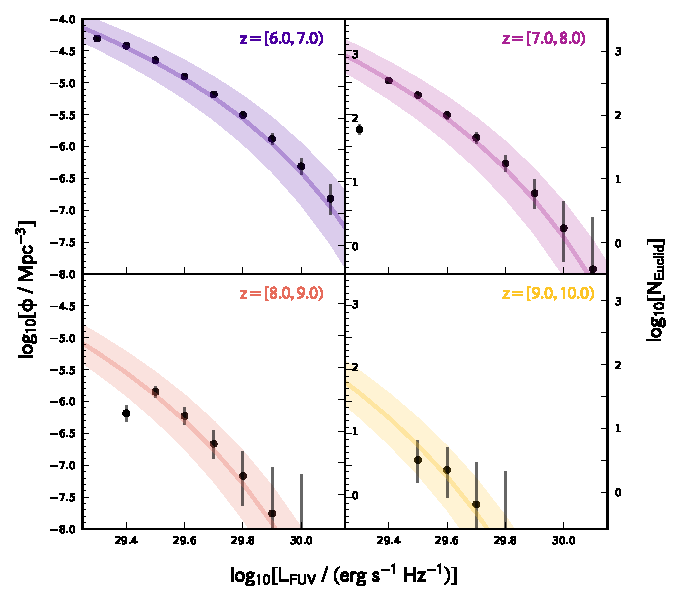
\includegraphics[width=0.5\textwidth]{figures/density/LF.pdf}
	\caption{\textcolor{red}{*** PLACEHOLDER; to do: double check it's correct. Add observed binned LFs where applicable. Add some literature constraints ***}{ Predicted luminosity functions in $\rm z = [6, 10)$ of galaxies accessible for Euclid DEEP survey assuming $\rm 10\sigma$ detection at $\rm H < 25.3$. The black points are the predicted binned luminosity function, the solid line shows the \textsc{FLARES} luminosity function constraints \textcolor{red}{CITE ASWIN} and the shaded region shows the \textsc{FLARES} luminosity function at the lower and upper bound of each redshift bin.}
	\label{fig:density:lfs}}
\end{figure}


\begin{figure}
	\centering
	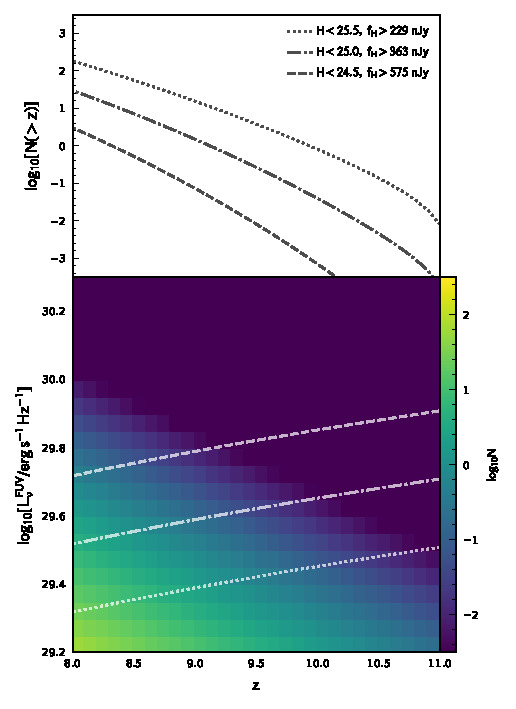
\includegraphics[width=0.5\textwidth]{figures/density/density.pdf}
	\caption{\textcolor{red}{*** PLACEHOLDER; to do: double check it's correct. Fix colorbar label *** }{Predicted cumulative numbers of sources in $\rm z = [8, 11)$ of galaxies accessible for Euclid DEEP survey. Three limiting magnitudes are considered.} 
	\label{fig:density:lfe}}
\end{figure}